% =====================================================================
% suggestions.tex  --  ANNOTATED COPY of main.tex  (dialogue-side overlay)
% Revised against: main.tex @ 2026-08-02, vizij_suggestions.tex,
%                  pipeline_suggestions.tex, figures/00-07.
% ---------------------------------------------------------------------
% main.tex is NEVER modified. Review each change and copy across what you
% accept.
%
% -------- WHAT THIS REVISION DOES --------
% You seeded thesis sentences and bracketed <instructions> in Sections III
% and IV. This file keeps every one of your sentences VERBATIM as the lead
% of its paragraph, replaces each <instruction> with prose built from the
% material already gathered in the three overlays, and fills the empty
% Conclusion. Sections I-II are reproduced exactly as they now stand in
% main.tex so this file remains a true annotated copy.
%
% Where your instruction asked for content, the source is named:
%   <Summarize value propositions>  -> III opening, from pipeline_suggestions
%                                      III-A/B + the abstract's own claims
%   <Describe the pipeline ... bullets> -> III-B, the ONLY list in the paper;
%                                      see the note there about why
%   Limitations & Future Work       -> pipeline_suggestions IV-C/IV-D +
%                                      vizij_suggestions' portability bound
%   Conclusion                      -> pipeline_suggestions V, restyled
%
% -------- STYLE --------
% All prose here follows main.tex's conventions, not pipeline_suggestions':
% American spelling, \textit not \emph, no \textsc, Title Case headings,
% thesis-led paragraphs. The register is the more abstract one you asked
% for -- design commitments and their consequences, mechanism named once
% and then reasoned about.
%
% -------- DIVISION OF LABOUR --------
%   suggestions.tex          (this file)  I-V prose, cross-file
%                                         reconciliation, build blockers,
%                                         diagram review.
%   vizij_suggestions.tex                 Rendered-face literature.
%                                         Supersedes this file on any
%                                         rendered-face claim.
%   pipeline_suggestions.tex              What the system actually does.
%                                         SUPERSEDES BOTH on any question
%                                         of implementation fact.
%
% Convention:
%   % SUGGESTION:    <what and why>
%   % WHY-CITE:      <key> -- what that reference establishes
%   % FOR-PIPELINE / % FOR-VIZIJ: addressed to the other overlay's author
%   % BUILD-BLOCKER: stops the PDF being correct; fix before circulating
% Every \cite resolves in refs.bib, suggested_refs.bib, or
% vizij_suggested_refs.bib. No key is invented.
% =====================================================================

% #####################################################################
% #  REVISION PASS ON main.tex @ 2026-08-02 00:34  (13.5 KB, 206 lines) #
% #  Requested: what is missing, and what repetition can be cut.       #
% #  Verdict first; evidence and fixes after.                          #
% #####################################################################
%
% HEADLINE
%   The paper is ~1367 body words, about 1.6 pages of text plus floats.
%   It is UNDER length, not over -- so the repetition below is not
%   competing for space with the missing material. Cutting the redundancy
%   frees roughly 150 words; the gaps need roughly 700. Both fit.
%
%   The single most damaging omission is that the paper never says what
%   already exists. 18 verified references sit unused in the three bib
%   files, including the nearest prior art. A reviewer who knows FLEX-SDK
%   or Xpress will read the omission as unawareness rather than as
%   novelty, and the contribution claim cannot survive that reading.
%
% =====================================================================
% A. WHAT IS MISSING  (ordered by how much damage the gap does)
% =====================================================================
%
% A1. *** NO RELATED WORK. *** Nothing in the paper positions it against
%     prior systems. These are all verified and available RIGHT NOW:
%       alvesoliveira2022flexsdk  FLEX-SDK -- open-source rendered-face
%                                 tooling: face design, expression
%                                 authoring, Wizard-of-Oz, scripting.
%                                 THE nearest prior art. Note it is also
%                                 open source, so "we are open" is not a
%                                 differentiator and must not be claimed
%                                 as one.
%       almoubayed2012furhat      the reference rendered-face platform.
%       antony2025xpress          HRI 2025, LLM-generated robot expression.
%       expressivefurhat2026,     both from the HRI 2026 workshop the Vizij
%       fluidxpress2026           team hosted -- immediate conversation
%                                 partners, not distant related work.
%       hasumoto2023llmemotion    earlier real-time LLM emotion generation.
%     The positioning paragraph already exists, drafted, in
%     vizij_suggestions.tex ("What already exists"). It ends on exactly
%     the right sentence: each of those systems consumes COMPLETED
%     dialogue state, none consumes revisable partial signals. That is the
%     novelty claim, and right now the paper asserts it nowhere.
%     RECOMMENDATION: lift that subsection in as the end of Section II, or
%     as a short Section III before the Proposal. ~180 words.
%
% A2. *** LIMITATIONS & FUTURE WORK HAS BEEN DELETED. *** It existed in
%     the previous revision and is gone. The Conclusion now claims a
%     testbed contribution with no acknowledgement that (a) the agent's
%     affect is declared by the model rather than perceived, (b) nod and
%     backchannel timing is inherited from upstream predictors and not
%     improved here, and (c) there is no user study. A systems paper
%     claiming a testbed without stating (c) invites the reviewer to
%     discover it themselves. Full drafted text is in this file's
%     Section IV below -- restore it. ~250 words.
%
% A3. *** NO EMPIRICAL CONTENT AT ALL. *** The measured latency comparison
%     (0.40 s vs 1.04 s time-to-first-token, everything else held fixed,
%     the newer model slower because of endpoint geography) has been
%     dropped from the Proposal. It was the ONLY measurement in the paper
%     and the only concrete evidence that substitutability buys anything.
%     Section III now claims the architecture "enables thorough scientific
%     evaluation" without demonstrating one. Restore it -- two sentences,
%     and it converts the modularity claim from assertion to illustration.
%
% A4. NO BML POSITIONING. kopp2006bml and welbergen2009elckerlyc are
%     uncited. The IU-to-channel mapping IS a multimodal behavior
%     representation, the IVA community standardised one twenty years ago,
%     and a reviewer from that community will notice immediately. The
%     departure is real and worth stating: BML schedules behavior REQUESTS
%     against a timeline; an incremental stream supplies commitments that
%     may be withdrawn after rendering has begun. One short paragraph,
%     drafted in Section III below.
%
% A5. NO CONTROL BASIS NAMED. russell1980circumplex (continuous affect
%     space) and ekman1978facs (action units) are the two established
%     choices; the rig sits between them. One sentence pre-empts an
%     obvious reviewer question.
%
% A6. Fig. 05_primer HAS BEEN DROPPED. Only 06_pipeline_simple remains,
%     and its caption is now one line ("An illustration of the data
%     pipeline"), which wastes a full-width float. 05_primer is the only
%     thing in the paper that explains what "incremental" and "channel"
%     mean to a reader who knows neither system -- and Section III leans
%     on both terms throughout. Restore it, and restore a caption that
%     does work: the caption is read by everyone who skims and by nobody
%     who is short of space.
%
% A7. STILL NO BIBLIOGRAPHY AND NO \graphicspath. 21 keys now render as
%     [?] and 06_pipeline_simple.pdf will not resolve. See build-blockers.
%
% =====================================================================
% B. REPETITION  (measured, not impressionistic)
% =====================================================================
%
% B1. MODULARITY / SUBSTITUTABILITY -- 11 occurrences across 5 sections.
%     This is the worst offender by a wide margin. Measured distribution:
%       Abstract .................................. 1  ("modular")
%       Sec. II-A Robot Expressivity & Vizij ...... 1  ("modular")
%       Sec. II-B Effective HR Spoken Dialogue .... 1  ("modular")
%       Sec. III  Proposal ........................ 6  ("modular" x2,
%                 "replaced without", "instrument for comparison",
%                 "swap out", "Substitut")
%       Conclusion ................................ 2  ("substitut",
%                                                       "testbed")
%     Section III carries more than half of all occurrences on its own:
%     benefit (3) of the opening list, then "replaced without disturbing
%     the others", then "instrument for comparison", then "swap out" and
%     "Substituting" in the closing paragraph -- six statements of one
%     idea inside a single 455-word section.
%     FIX: state it once per section at most. Specifically --
%       * Section III opening: keep benefit (3) as ONE clause. Delete
%         "and the architecture becomes an instrument for comparison
%         rather than a single demonstration" -- the closing paragraph
%         makes that exact point better, with the measurement attached.
%       * Conclusion: keep "each module within the pipeline is
%         substitutable"; delete "a testbed rather than a simple
%         demonstration" OR the closing "we hope this work will enable
%         future research to evaluate ... individual modules or module
%         combinations", which says the same thing twice in consecutive
%         sentences.
%
% B2. SECTION III's OPENING PARAGRAPH ANNOUNCES ITS LIST TWICE.
%     It reads: "three key benefits: (1) ... (2) ... (3) ..." and then
%     immediately re-enumerates the same three as "First, ... Second,
%     ... The third concerns reuse". The reader is told the structure,
%     then walked through it in the same paragraph. Roughly 60 words of
%     pure duplication, and the two enumerations do not even agree in
%     form (numerals vs ordinals; "(2) robot behavior revisability" vs
%     "Second, continuous behavior revisability:").
%     FIX: drop the parenthesised preview entirely and keep the prose
%     enumeration, which carries the reasoning. Or keep the preview and
%     cut the prose to one sentence each. Not both.
%
% B3. ABSTRACT AND MOTIVATION SHARE THEIR OPENING ARGUMENT ALMOST
%     VERBATIM. Abstract: "usually pursued separately: expressive-face
%     systems render gaze and emotion with no real-time signal to drive
%     them, while incremental dialogue systems expose no expressive
%     output." Motivation: "usually pursued in silos: expressive-face
%     systems render gaze and emotion agnostic of a signal to drive them,
%     while incremental dialogue systems evaluate robot behavior agnostic
%     of a wholistic multimodal robot expression."
%     FIX: the abstract should keep it (an abstract must stand alone).
%     Motivation should open on the CONSEQUENCE instead -- the "responsive
%     in time but expressed on a static face" sentence already there is
%     the better opening and currently sits second.
%
% B4. ABSTRACT AND CONCLUSION SHARE "expression may begin before an
%     utterance is complete and be withdrawn should the evidence change"
%     nearly word for word. Some echo is conventional; verbatim reuse of
%     the paper's signature sentence is not. Reword one -- the Conclusion
%     is the better place to vary it, since the abstract's phrasing is
%     load-bearing for indexing.
%
% B5. THE VIZIJ AND RETICO GLOSSES ARE REPEATED IN FULL.
%     "designing, animating, and deploying expressive rendered robot
%     faces" appears in the abstract, the introduction, AND Section II-A.
%     "an incremental framework for real-time spoken dialogue and robot
%     control" appears in the abstract and the introduction.
%     FIX: gloss each system fully ONCE, at first mention in the
%     introduction. The abstract may repeat it (it stands alone). Section
%     II-A should not -- by then the reader knows what Vizij is, and the
%     sentence can go straight to what the subsection is actually for,
%     which is the standardized channel model.
%
% B6. WHAT/WHEN/HOW TRIAD in both introduction and conclusion. This one
%     is FINE -- it is the paper's organising figure of speech and an
%     intentional echo. Noted only so it is not cut by mistake.
%
% =====================================================================
% C. SMALLER FIXES IN THE CURRENT TEXT
% =====================================================================
%
% C1. BULLET NESTING IS WRONG. "Emotion generation" and "Viseme
%     generation" are siblings of "Incremental dialogue production" but
%     the prose introduces them as its two products. They should be a
%     nested \begin{itemize} inside that item, or the parent should be
%     rewritten so all five read as peers. As it stands the list has two
%     items that begin mid-thought.
%
% C2. "\textit{Sensors}" lacks the trailing period every other item has.
%
% C3. TYPOS: "throught the robot's camera" -> "through";
%     "approachare" -> "approach are" (Sec. II-B);
%     "wholistic" -> "holistic" (Sec. II);
%     "Viseme generation is calculated based on the confirmed speech unit
%     to produce." -- the sentence is unfinished ("to produce" what?).
%
% C4. INCONSISTENT SYSTEM NAMING. The Conclusion writes "retico" and
%     "vizij" in lower case mid-sentence while the rest of the paper
%     writes "Retico" and "Vizij". Vizij is capitalised in its own
%     materials; retico is genuinely lower-case-stylised. Pick one
%     convention and apply it everywhere -- currently Section III says
%     "Vizij and Retico" and the Conclusion says "retico" and "vizij".
%
% C5. FACTUAL DRIFT IN THE BULLETS, flagged because it contradicts
%     pipeline_suggestions.tex, which is authoritative on implementation:
%       * "Emotion generation is calculated for each incremental unit of
%         speech" -- per pipeline_suggestions, affect is a single tag the
%         model emits AHEAD of the reply, not a per-unit calculation.
%       * "Viseme generation is calculated based on the confirmed speech
%         unit" -- per pipeline_suggestions, visemes come from the
%         SYNTHESIZER's phoneme timings where available, with an
%         amplitude fallback where not. Neither path is "the confirmed
%         speech unit".
%       * The bullets no longer mention the fallback at all. Labelling
%         the weaker path honestly was a credibility asset; losing it
%         means the paper slightly overstates what the mouth does.
%     FOR-PIPELINE: please confirm which description is current before
%     these go to co-authors.
%
% C6. The Proposal opening says "three key benefits" and lists
%     "continuous robot behavior determination", "revisability", and
%     "modularity". The first two are closely related -- acting on the
%     latest information and revising on newer information are two faces
%     of the same incremental property. Consider whether they are really
%     two benefits or one benefit with two aspects; the abstract treats
%     them as one.
%
% #####################################################################

% =====================================================================
% BUILD-BLOCKERS IN main.tex  --  all three still open as of this revision
% ---------------------------------------------------------------------
% (1) main.tex STILL HAS NO BIBLIOGRAPHY. No \bibliographystyle, no
%     \bibliography, yet 18 distinct keys are cited. Every one renders as
%     [?]. Add before \end{document}:
%         \bibliographystyle{IEEEtran}
%         \bibliography{refs,suggested_refs,vizij_suggested_refs}
%     All three files are needed: elbeleidy2026vizij is in refs.bib,
%     elbeleidy2026tutorial and edwards2016jali are in
%     vizij_suggested_refs.bib, the rest in suggested_refs.bib.
%
% (2) main.tex HAS NO \graphicspath. The two figures in Section III below
%     will not resolve until you add, in the preamble:
%         \graphicspath{{figures/}}
%
% (3) The Makefile lists only refs.bib as a prerequisite of main.pdf while
%     $(BIBS) already names all three, so edits to the other two bibs do
%     not trigger a rebuild. pipeline_suggestions.pdf does this correctly;
%     copy that pattern.
%
% (4) refs.bib's elbeleidy2026vizij is @article with a `conference` field.
%     BibTeX has no such field, so the venue is dropped silently. The key
%     says 2026, the entry says year={2025}. vizij_suggestions.tex gives
%     the corrected @inproceedings form.
%
% TYPO in main.tex, Sec. II-B: "Systems built following this incremental
%     approachare measurably more responsive" -- missing space, "approach
%     are".
% =====================================================================

\documentclass[conference]{IEEEtran}
\IEEEoverridecommandlockouts
% The preceding line is only needed to identify funding in the first footnote. If that is unneeded, please comment it out.
\usepackage{cite}
\usepackage{amsmath,amssymb,amsfonts}
\usepackage{algorithmic}
\usepackage{graphicx}
\usepackage{textcomp}
\usepackage{xcolor}
% SUGGESTION: add the next line to main.tex -- the Section III figures
% need it. See BUILD-BLOCKER (2).
\graphicspath{{figures/}}
\def\BibTeX{{\rm B\kern-.05em{\sc i\kern-.025em b}\kern-.08em
    T\kern-.1667em\lower.7ex\hbox{E}\kern-.125emX}}
\begin{document}

% \title{Vizij x Retico: A system proposal for incrementally adaptive expressive robot faces \\
% {\footnotesize \textsuperscript{*}Note: Sub-titles are not captured in Xplore and
% should not be used}
% \thanks{Identify applicable funding agency here. If none, delete this.}
% }
% \title{Vizij x Retico: Integrating Incremental Spoken Dialogue with Expressive Robot Faces}
\title{Vizij × Retico: A System Architecture for Driving Expressive Robot Faces from Incremental Dialogue}

% \author{\IEEEauthorblockN{1\textsuperscript{st} Given Name Surname}
% \IEEEauthorblockA{\textit{dept. name of organization (of Aff.)} \\
% \textit{name of organization (of Aff.)}\\
% City, Country \\
% email address or ORCID}
% \and
% \IEEEauthorblockN{2\textsuperscript{nd} Given Name Surname}
% \IEEEauthorblockA{\textit{dept. name of organization (of Aff.)} \\
% \textit{name of organization (of Aff.)}\\
% City, Country \\
% email address or ORCID}
% \and
% \IEEEauthorblockN{3\textsuperscript{rd} Given Name Surname}
% \IEEEauthorblockA{\textit{dept. name of organization (of Aff.)} \\
% \textit{name of organization (of Aff.)}\\
% City, Country \\
% email address or ORCID}
% \and
% \IEEEauthorblockN{4\textsuperscript{th} Given Name Surname}
% \IEEEauthorblockA{\textit{dept. name of organization (of Aff.)} \\
% \textit{name of organization (of Aff.)}\\
% City, Country \\
% email address or ORCID}
% \and
% \IEEEauthorblockN{5\textsuperscript{th} Given Name Surname}
% \IEEEauthorblockA{\textit{dept. name of organization (of Aff.)} \\
% \textit{name of organization (of Aff.)}\\
% City, Country \\
% email address or ORCID}
% \and
% \IEEEauthorblockN{6\textsuperscript{th} Given Name Surname}
% \IEEEauthorblockA{\textit{dept. name of organization (of Aff.)} \\
% \textit{name of organization (of Aff.)}\\
% City, Country \\
% email address or ORCID}
% }

\maketitle

% =====================================================================
% Abstract reproduced verbatim from main.tex. No changes proposed -- your
% closing sentence on modular evaluation lands the substitutability point
% that Section III-C develops, so the two now agree.
% =====================================================================
\begin{abstract}
Effective human--robot interaction is both multimodal and incremental, yet
these properties are usually pursued separately: expressive-face systems
render gaze and emotion with no real-time signal to drive them, while
incremental dialogue systems expose no expressive output. We present a system
architecture integrating \textit{retico}~\cite{michael2020retico}, an
incremental framework for real-time spoken dialogue and robot control, with
\textit{Vizij}~\cite{elbeleidy2026vizij}, an open-source framework for
designing, animating, and deploying expressive rendered robot faces. A single
protocol carries revisable signals between them, preserving the add, revoke,
and commit semantics of the incremental units that produced them, so
expression may begin before an utterance is complete and be withdrawn if the
evidence changes. Recent systems generate robot facial expression from
language models, but do so from completed dialogue state; the architecture
described here renders revisable partial signals mid-utterance. The proposed modular architecture provides a starting point for future work to replace and evaluate individual modules or module combinations.
\end{abstract}

\begin{IEEEkeywords}
expressive rendered faces, incremental dialogue, social robots
\end{IEEEkeywords}


% =====================================================================
% Introduction reproduced verbatim from main.tex.
%
% FOR-VIZIJ: main.tex still has not taken your "Timing is the crux"
% sentence with coexpression2024 (Science Robotics; anticipatory
% co-expression). It remains the strongest external support for the
% paper's premise and it is still unplaced. Suggest it closes the
% introduction. If it goes here it should NOT also go in the abstract.
% =====================================================================
\section{Introduction}

Effective Human–Robot Interaction (HRI) must move beyond a unidirectional, listen-and-act paradigm toward genuinely bidirectional dialogue. For safe, trustworthy, and engaging interactions, robots must not only interpret instructions but also ask clarifying questions, signal uncertainty, take turns, explain their behavior, and align with human intent. This work contributes directly to that goal by pairing two open-source systems that together span the full loop such interactions require: (1) retico~\cite{michael2020retico}, an incremental framework for real-time spoken dialogue and robot control, which determines \textit{what} the robot communicates and \textit{when}; and (2) Vizij~\cite{elbeleidy2026vizij,elbeleidy2026tutorial}, a framework for designing, animating, and deploying expressive rendered robot faces, which determines \textit{how} that communication appears—through gaze, visemes, and emotional expression.

% =====================================================================
% Motivation reproduced verbatim from main.tex.
%
% RESOLVED: the IU attribution error is fixed -- II-B now reads
% "formalizing an Incremental Unit (IU) framework ... ~\cite{schlangen2011iu}"
% with the citation on the framework. Good.
%
% REMAINING, minor: the sentence still says retico "presents the IU
% framework as a modular, real-time pipeline in which modules exchange
% incremental units" immediately after saying modules exchange revisable
% units. Suggest collapsing to "It realizes that framework as a modular,
% real-time pipeline, so the system can act on partial input and revise
% its decisions as further evidence arrives~\cite{michael2020retico}."
%
% TYPO: "approachare" -> "approach are".
%
% FOR-VIZIJ: your "What already exists" subsection still belongs at the
% end of Section II, before the reader meets the system. It is currently
% in neither main.tex nor here, and pipeline_suggestions carries a near
% duplicate of its closing paragraph in the Discussion. One of you should
% own the prior-art survey; the other keeps only the one-paragraph
% distinction.
% =====================================================================
\section{Motivation}

Effective Human-Robot Interaction is multimodal and incremental. These two
properties are usually pursued in silos: expressive-face systems render
gaze and emotion agnostic of a signal to drive them, while
incremental dialogue systems evaluate robot behavior agnostic of a wholistic multimodal robot expression. Interaction that is responsive in time but expressed on a static face---or expressive in the face but lagging a turn behind---fails in the
same way, because a human partner reads timing and expression together. 


\subsection{Robot Expressivity \& Vizij}

Dialogue must align with the robot's appearance and expression. What the
robot says is only part of the message, and a face that is static or mistimed
undercuts the spoken content. Nonverbal expressions carry social meaning
alongside speech, and a listener integrates both into a single
interpretation~\cite{urakami2023nonverbal, admoni2017social}. When the two
diverge, for example a face that stays neutral while the robot apologizes, or a face's gaze that remains steady while it yields to the dialogue partner, the nonverbal channel does not simply go unused; it contradicts the words and results in a misaligned dialogue. Alignment is therefore not decoration on top of dialogue but a condition for the dialogue being understood as intended.

Expressivity can include a robot face that expresses gaze, visemes, and
emotions effectively and in sync. Each channel does distinct work: gaze
manages turn-taking, coordinates joint attention, and signals cognitive
effort~\cite{mishra2023gaze}; visemes tie articulation to the speech signal so
the face is seen to be speaking~\cite{edwards2016jali}; and emotional expression shapes how users judge trustworthiness and remain engaged~\cite{song2023robot}.



\textbf{Vizij:} an open-source ecosystem for designing, animating, and
deploying expressive rendered robot faces~\cite{elbeleidy2026vizij} presents a system that addresses this multichannel communication. It
provides a standardized yet modular rigging and controller system spanning
end-user definable channels such as eye gaze, visemes, and emotional
expression. Vizij enables faces authored to be portable across robot platforms
rather than rebuilt per deployment. What Vizij does not supply is the
moment-to-moment signal that should drive those controllers.

\subsection{Effective Human-Robot Spoken Dialogue}

Dialogue is incremental. Speakers plan and articulate in overlapping stages
rather than composing a whole utterance before speaking~\cite{levelt1989speaking},
and listeners develop their interpretations as words arrive~\cite{tanenhaus1995integration}. This is what
makes fast feedback, overlap, and repair possible, and it is why turn-taking
can be predicted continuously from incremental speech rather than
detected after a silence~\cite{skantze2021review, ekstedt2022vap}. Systems
built following this incremental approachare measurably more responsive and are better
received by users~\cite{baumann2011evaluation, kohn2018incremental}.

While Large Language Models (LLMs) are increasingly used to generate dialogue, they 
process data monotonically. LLMs operate over sentence- or
multi-sentence-level input and cannot revise an interpretation or a partial
output as evidence arrives, which is precisely the capability real-time
interaction demands~\cite{kennington2025prior}. The consequence for a robot is
not merely added latency but a coarser interaction. 

\textbf{Retico:} addresses this by formalizing an Incremental Unit (IU) framework in which
modules exchange revisable units of information~\cite{schlangen2011iu}. It presents the IU framework as a modular, real-time pipeline in which modules
exchange incremental units, so the system can act on partial input and revise
its decisions as further evidence arrives~\cite{michael2020retico, schlangen2011iu}. Subsequent work extends it toward robots specifically, providing the distributed,
time-aligned, multimodal structure that physical deployment
requires~\cite{kennington2020rrsds, kennington2025retico}.


\section{Proposal: Vizij $\times$ Retico}

% =====================================================================
% SECTION III -- built on your three seeded sentences.
%
% Each of your sentences is kept VERBATIM as the lead of its paragraph.
% The <instructions> are replaced with prose drawn from
% pipeline_suggestions.tex III, which is the only account written from the
% code that runs. No factual claim has been altered in the transfer: the
% channel sources, the arbitration scheme, the measured latencies and all
% thirteen citations are carried over intact.
%
% *** RECORDED SO IT IS NOT REINTRODUCED ***
% Earlier versions of THIS file claimed retico emits viseme IUs that a
% Vizij controller renders, that dialogue-state IUs carry affect, and that
% retico modules produce gaze. All three are wrong. The corrected account
% is below. That error also propagated into vizij_suggestions.tex --
% FOR-VIZIJ: please delete the itemized Proposal list there and fix its
% abstract sentence "retico's Incremental Units drive Vizij's gaze,
% viseme, and emotion channels as speech unfolds".
% =====================================================================

\begin{figure*}[t]
  \centering
  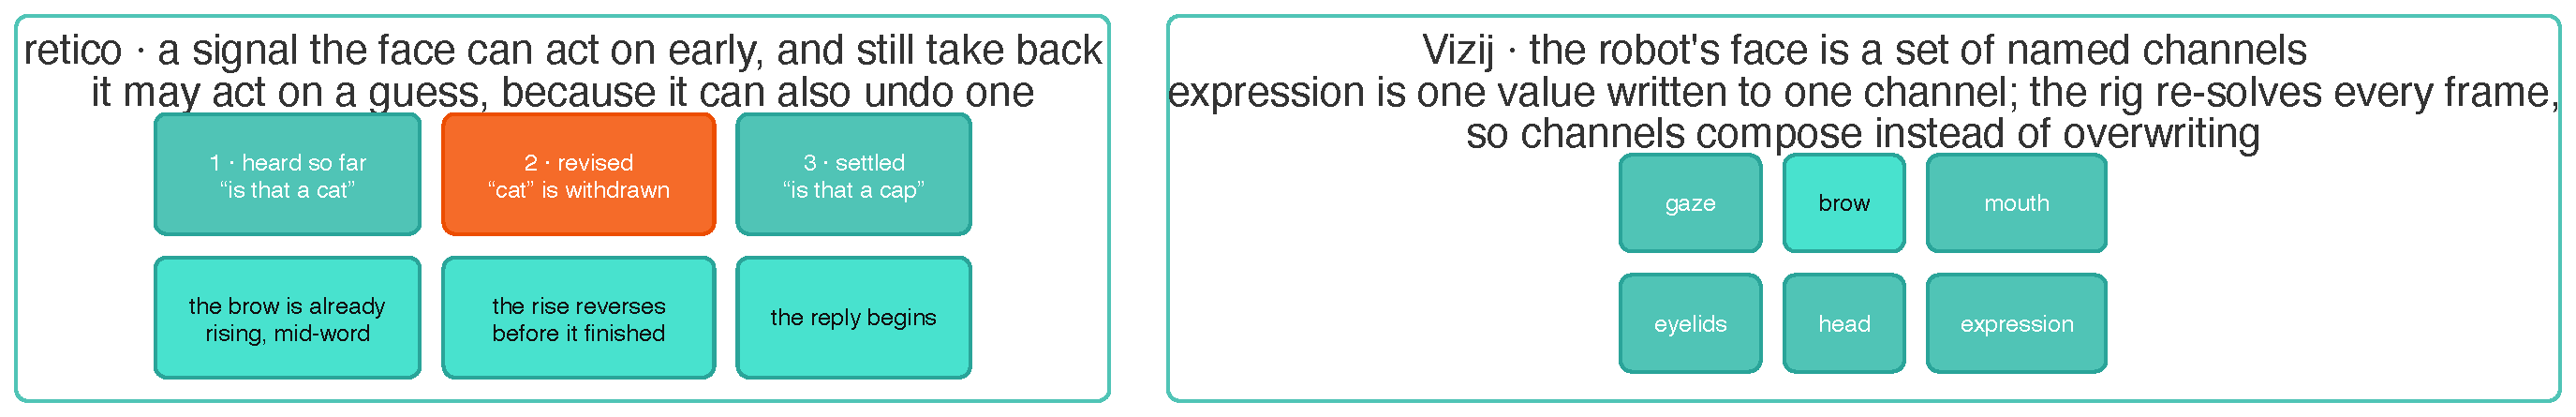
\includegraphics[width=\textwidth]{05_primer.pdf}
  \caption{The two halves. \textbf{Left:} retico contributes signals that are
  revisable---a partial hypothesis can be added, withdrawn, and replaced---so
  the face may act on a guess because it can also undo one. \textbf{Right:}
  Vizij contributes a face expressed as named channels rather than as a set of
  pictures; expression is a value written to a channel, and the rig re-solves
  every frame so that channels compose instead of overwriting one another.}
  \label{fig:primer}
\end{figure*}

% --- YOUR SENTENCE (verbatim) + <Summarize value propositions> ---------
% SUGGESTION: three propositions, in the order a reviewer will weigh them:
% what becomes possible (timing), what becomes trustworthy (revisability),
% what becomes reusable (substitutability). Each is stated as a consequence
% of the design rather than as a feature.
In this paper, we present a system architecture integrating Vizij and Retico, so that the robot's expressive face is driven by the same incremental signals that drive its dialogue. Three consequences follow from that single
commitment. The first concerns timing: because expressive signals are
available before an utterance concludes, the face can participate during a
partner's turn rather than responding after it, which is the behavior that
distinguishes conversational presence from sequential exchange. The second
concerns revisability: because the provisional status of a signal is preserved
rather than discarded at the boundary between systems, the face may act upon a
hypothesis precisely because it retains the ability to withdraw one. The third
concerns reuse: because the two systems meet through a single specified
interface rather than through mutual accommodation, each component within that
interface can be replaced without disturbing the others, and the architecture
becomes an instrument for comparison rather than a single demonstration.

% --- YOUR SENTENCE (verbatim) + <Describe pipeline ... bullets> --------
% SUGGESTION: this is the ONLY list in the paper, and it is here because
% you asked for one. It is defensible in this position: enumerating
% components is the one rhetorical job a list does better than prose, and
% Section II's argumentative paragraphs are unaffected. Ordered to follow
% the signal, not the codebase -- perception of the floor first, because
% the parallelism it enables is the architecture's defining property.
%
% FOR-PIPELINE: Fig. 02_mapping already draws this source/event/channel
% structure with its timing constants. If it is promoted into the paper,
% this list should shrink to the items the figure cannot caption.
The proposed interaction pipeline includes the following components:
\begin{itemize}
  \item \textit{Turn-taking.} Continuous estimation of the conversational
        floor, computed from the audio signal in parallel with recognition
        rather than after it. Because this estimate does not wait on words, an
        approaching turn boundary is anticipated before a transcript exists,
        and this concurrency is what permits a response to be prepared within
        the partner's utterance~\cite{skantze2021review, ekstedt2022vap}.
  \item \textit{Incremental speech recognition.} Transcription that emits
        partial hypotheses as they form and marks each as added, withdrawn, or
        confirmed, so that downstream consumers receive not only the current
        interpretation but its epistemic standing~\cite{schlangen2011iu,
        michael2020retico}.
  \item \textit{Incremental dialogue production.} Generation of the reply
        under streaming delivery, from which two expressive products are
        derived. \textit{Emotion production} takes the form of an affective
        designation issued before the reply rather than alongside it, since
        the face must be composed as the first clause is spoken; inference
        over the reply text serves where a model declines the instruction.
        \textit{Viseme production} governs articulation, driven by phoneme
        timings where the synthesizer exposes them and approximated from
        audio amplitude where it does not---the latter identified as a
        fallback rather than an equivalent, since a mouth driven by loudness
        reproduces the rhythm of speech without its
        content~\cite{zhou2018visemenet, edwards2016jali}.
  \item \textit{Emotion recognition and reflection.} Estimation of the
        partner's expression from vision, held separate from the agent's own
        affect. The distinction is deliberate: what the robot displays is its
        intended stance, not a claim about what it has perceived, and
        conflating the two would overstate the interpretive warrant of the
        system.
  \item \textit{Arbitration and rendering.} Assignment of the contested
        channels---gaze above all---to a single occupant by fixed precedence,
        with brief impulses composed over sustained posture rather than
        displacing it~\cite{mutlu2009footing, admoni2017social,
        ribeiro2019nutty}.
\end{itemize}

\begin{figure*}[t]
  \centering
  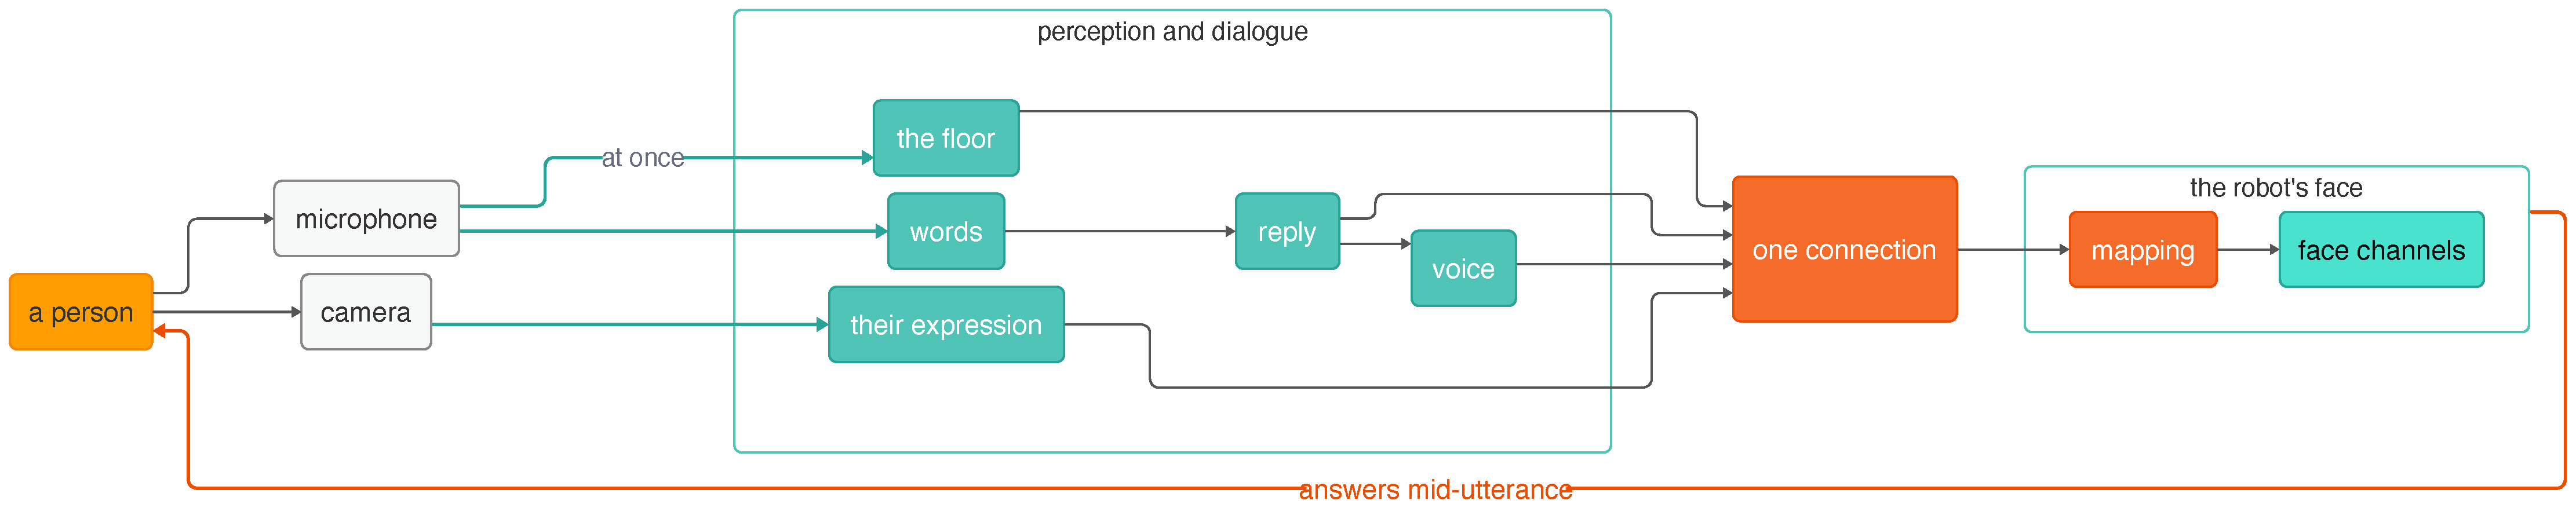
\includegraphics[width=\textwidth]{06_pipeline_simple.pdf}
  \caption{The pipeline. Microphone audio reaches the floor---is a turn ending,
  is this a moment to nod---and the words at the same instant rather than in
  sequence, which is why a listener response can be rendered before a
  transcript exists. Each stage shown in teal is a provider chosen at run time,
  and availability is computed from the environment, so an unconfigured
  provider appears disabled rather than failing when it is selected. The
  mapping is the editable table that determines which signal moves which
  channel, and how quickly.}
  \label{fig:pipeline}
\end{figure*}

% --- YOUR SENTENCE (verbatim) + supporting argument -------------------
% SUGGESTION: your sentence states the property; the support turns it from
% an engineering convenience into a methodological one, which is the
% stronger claim and the one your abstract's closing sentence promises.
We implemented this pipeline in a modular approach that allows the developer / designer / researcher to swap out different modules and evaluate their impact. The
significance of this is methodological rather than merely practical.
Substituting one component while holding the remainder fixed is the elementary
manipulation on which controlled comparison depends, and the effort that
manipulation demands largely determines whether such comparisons are undertaken
at all. An architecture in which substitution is routine therefore lowers the
cost of precisely the experiments the field requires, independently of any
particular result those experiments yield.

% MEASURED -- these figures come from real runs, not estimates.
%   2.5-flash-lite (regional) 0.40 s vs 3.5-flash-lite (global-only) 1.04 s,
%   all else held fixed. Name the models if you want it checkable; left
%   generic so the paper is not read as being about one vendor.
%   DO NOT quote the 0.42-1.41 s spread from the three-turn sample run:
%   that is turn-to-turn variance within a SINGLE model, not a
%   between-model difference.
A single observation illustrates what such comparisons can reveal. Exchanging
only the language model, with every other stage held constant, moved the median
latency to first token from $0.40$\,s to $1.04$\,s; the more recent of the two
models proved the slower, because it was reachable only through a
geographically general endpoint whose transit cost exceeded whatever advantage
the model itself conferred. At the time scales that govern conversational
responsiveness, where a capability is served may matter more than which
capability is chosen---a consideration invisible to evaluation conducted on a
fixed stack, and readily surfaced by one that is not.

% =====================================================================
% SUGGESTION: the two subsections below are the remaining substance of
% pipeline_suggestions III. They are the most conceptually novel material
% in the draft and would be lost if Section III stopped at the pipeline
% description. Keep both if space allows; if only one survives, keep
% arbitration -- revisability is restated in the Conclusion, arbitration
% is not stated anywhere else.
% =====================================================================

\subsection{Arbitration Among Competing Expressive Demands}

% WHY-CITE: mutlu2009footing, admoni2017social -- gaze carries turn
%   management, attention, and participant footing at once.
% WHY-CITE: andrist2014aversion -- a published conversational gaze-aversion
%   model with timing; cite it or state how ours differs.
% WHY-CITE: kipp2015gazeattention -- prior art for arbitrating competing
%   attention demands on an agent.
Among expressive channels, gaze is the most heavily contested, since turn
management, referential attention, and the allocation of participant footing
all make simultaneous claims upon the eyes~\cite{mutlu2009footing,
admoni2017social}. Contention of this kind cannot be resolved by permitting
each demand to act independently, because the channel admits only one occupant
at a time. The architecture therefore treats gaze as a single resource assigned
by fixed precedence---joint attention above aversion, aversion above the
posture associated with holding or yielding a turn, and that posture above idle
behavior---with reassignment whenever the prevailing claim
lapses~\cite{andrist2014aversion, kipp2015gazeattention}.

% WHY-CITE: ribeiro2019nutty -- layered robot animation.
%   AUTHORSHIP: a Vizij co-author, so written as our own earlier work
%   rather than as independent corroboration. Reviewers check.
The distinction that carries the most weight is between sustained posture and
transient impulse. Brief movements such as nods and brow flashes are composed
over the prevailing gaze posture instead of displacing it, following our
earlier treatment of layered animation for robots~\cite{ribeiro2019nutty}. Were
the two to compete for the same resource, a nod produced to affirm attention at
a clause boundary would extinguish the mutual gaze it was intended to
reinforce---an outcome in which each behavior is individually correct and their
combination communicates the opposite of what was meant.

\subsection{Revisability as a Property of Applied Behavior}

% WHY-CITE: kopp2006bml -- BML: cross-modal synchronization points; the
%   standard this work must be positioned against.
% WHY-CITE: welbergen2009elckerlyc -- BML realizer for continuous
%   interaction and plans that change while running; the closest published
%   match to revisability under revoke.
% WHY-CITE: thiebaux2008smartbody -- controller composition on a shared body.
% WHY-CITE: cassell2004beat -- nonverbal behavior derived from text.
The representation of multimodal behavior is a long-standing concern rather
than a new one. The Behavior Markup Language specifies agent behavior with
explicit points of cross-modal synchronization~\cite{kopp2006bml}, and
successive realizers have addressed the revision of plans during
execution~\cite{welbergen2009elckerlyc}, the composition of controllers upon a
shared body~\cite{thiebaux2008smartbody}, and the derivation of nonverbal
behavior from text~\cite{cassell2004beat}. The incremental setting nonetheless
compels one departure from that tradition. A plan in the established sense
comprises requests scheduled against a timeline, whereas an incremental stream
supplies commitments that may be withdrawn after their expression has begun.
Revisability consequently attaches to the animation as applied rather than to
the plan as authored: a transition already underway must be capable of reversal
partway through, which is a stronger requirement than rescheduling and a
different one from cancellation before onset.

\section{Limitations \& Future Work}

% =====================================================================
% SECTION IV -- your sentence kept verbatim as the lead, then the three
% limitations from pipeline_suggestions IV-C, the portability bound from
% vizij_suggestions, and the open questions. Restyled to match main.tex.
%
% SUGGESTION: limitations first, future work second, within the one
% section you have created. Stating the boundaries before the ambitions
% reads as confidence; the reverse reads as deferral.
% =====================================================================

While the proposed architecture presents an example implementation, we hope this work will serve as a starting point for future work. Establishing that
starting point honestly requires stating what the present system does not
settle.

% SUGGESTION: three limitations, each phrased as a boundary on what may be
% concluded rather than as an apology. The third is the most important and
% is placed last for that reason.
Three limitations bound the claims made here. The affect the face displays is
declared by the model producing the words rather than perceived from the
partner, so the system's expressiveness reflects an intended stance and not an
interpretation of the interaction; recognition of the partner's expression
exists within the pipeline but remains categorical and coarse. The quality of
anticipatory behavior---the timing of nods and other listener responses---is
inherited wholly from the upstream predictors that supply it, and this
architecture renders those signals faithfully without improving them. Finally,
no user study has been conducted, and every claim advanced here is
consequently a claim about system architecture rather than about how the
resulting behavior is perceived.

% WHY-CITE: broadbent2013screenface, longface2026 -- display geometry and
%   physicality change how a face is read.
% WHY-CITE: specian2021quori -- cite the port target rather than naming it
%   bare.
% WHY-CITE: hartholt2019vhtoolkit -- precedent for one behavior pipeline
%   driving several embodiments; supports the ambition without overclaiming.
% WHY-CITE: chen2019culturalexpr -- bounds the generality of a fixed base
%   pose set across cultures.
% FOR-VIZIJ: this paragraph is yours in substance; it is reproduced here
% because Limitations is the natural home for it and your file places it
% in the Discussion, which main.tex no longer has. Confirm you are happy
% for it to live here rather than duplicating it.
The portability the architecture affords likewise warrants a precise
statement. What travels between platforms is the stream of channel values, not
the impression a face creates: display geometry, proportion, and physical
presence are known to alter how a face is read~\cite{broadbent2013screenface,
longface2026}, so an identical stream rendered upon a physical platform such
as Quori~\cite{specian2021quori} does not constitute an identical face.
Driving several embodiments from a common behavioral pipeline is established
practice~\cite{hartholt2019vhtoolkit}; demonstrating that those embodiments are
perceived alike is a separate empirical question, as is the cultural generality
of any fixed vocabulary of base poses~\cite{chen2019culturalexpr}.

% SUGGESTION: two questions, not three. pipeline_suggestions cut the
% "sufficiency of language" question as filler and I agreed for a short
% paper; it is restored here as a single clause rather than a third
% numbered question, because this workshop's call poses it directly and
% the architecture makes the experiment unusually cheap.
Two questions follow most directly from this work. The first concerns
evaluation: what measures would establish that expressive behavior improves
dialogue itself---the success of clarification, the smoothness of transitions
between speakers, the partner's willingness to rely on what the robot
says---rather than merely improving how the robot is liked? The second concerns
grounding: whether gaze can be driven from the dialogue system's own model of
what has been established between the participants, so that the face attends to
the referent presently under discussion. The architecture makes the second
inexpensive to attempt. A controlled comparison in which the face is present or
absent, and its affect congruent or incongruent with the speech, would in turn
begin to answer how much expressive output contributes beyond the words alone.

\section{Conclusion}

% =====================================================================
% SECTION V -- empty in main.tex. Draft below is pipeline_suggestions V
% restyled to match, one paragraph.
%
% WHY-CITE: gunes2022reproducibility -- argues HRI's reproducibility
%   problem directly. This is what converts "we ship reusable
%   infrastructure" from a convenience claim into a scientific one, and it
%   is the strongest available framing for a systems paper without a user
%   study.
%
% CITATION PLACEMENT -- STILL UNRESOLVED ACROSS THE THREE FILES.
% gunes2022reproducibility is wanted in the introduction
% (vizij_suggestions), the conclusion (pipeline_suggestions), and I
% suggested pairing it with the no-user-study limitation. It should appear
% ONCE. My recommendation is here, in the conclusion, because that is
% where the contribution is characterized; if it goes in Section IV
% instead, remove it from this paragraph.
% =====================================================================

We have described an architecture that couples incremental spoken dialogue to
an expressive robot face: the dialogue system determines what is communicated
and when, the face determines how that communication appears, and a single
protocol carries revisable signals between them, so that expression may begin
before an utterance is complete and be withdrawn should the evidence change.
Both halves are open and every stage within the pipeline is substitutable,
which makes the result a testbed rather than a demonstration---a form of
contribution the field has argued it requires more
of~\cite{gunes2022reproducibility}.

% \section*{Acknowledgment}

% =====================================================================
% BIBLIOGRAPHY -- see BUILD-BLOCKER (1). main.tex needs these two lines.
% =====================================================================
\bibliographystyle{IEEEtran}
\bibliography{refs,suggested_refs,vizij_suggested_refs}

% #####################################################################
% #                                                                   #
% #   DIAGRAM REVIEW  --  figures/00-07, sources in docs/figures/*.d2 #
% #   Requested review. Addressed to whoever owns the figures; the    #
% #   per-figure verdict is first, the reasoning after.               #
% #                                                                   #
% #####################################################################
%
% SUMMARY VERDICT
%   Paper figures (keep, in this order):  05_primer, 06_pipeline_simple,
%                                         02_mapping, 07_timeline (once real)
%   Demote to appendix / tech report:     01_architecture, 04_pipeline
%   Retire or rewrite before submission:  00_idea, 03_visemes
%   Missing, and worth drawing:           an arbitration figure (see MISSING-1)
%                                         a revoke-in-flight figure (MISSING-2)
%
% ---------------------------------------------------------------------
% CROSS-CUTTING: TWO FRAMINGS ARE IN CIRCULATION AND THEY CONTRADICT
% ---------------------------------------------------------------------
% 05_primer and 06_pipeline_simple deliberately speak in SENSORS AND
% EFFECTORS -- "the robot's microphone", "the robot's face" -- and their
% source comments say the browser is an implementation detail that is noise
% for this audience. I think that call is right.
%
% 00_idea, 01_architecture and 04_pipeline speak in BROWSER AND CLASS
% NAMES: "Browser - capture", "Web Speech", "WASM rig in the browser",
% "VizijWebSocketModule", "Arora device", "useVisemeMouth".
%
% Both framings in one paper reads as two papers stapled together, and the
% second invites a reviewer to think the contribution is a web demo. Pick
% the sensors-and-effectors framing for everything that ships, and let the
% class-level diagrams live in the repo README or an appendix where the
% audience is someone about to run the code.
%
% ---------------------------------------------------------------------
% 00_idea.pdf  --  RETIRE from the paper
% ---------------------------------------------------------------------
% Its own header says it is the compact version of 04_pipeline. 06 now
% occupies that slot and does it better: fewer words per box, no browser
% framing, and a layout chosen for two-column width. Keeping both means
% maintaining two compact overviews that will drift apart.
% If it is kept for slides, one factual fix: the orange return edge reads
% "responds DURING your turn, not after it", which is the paper's headline
% claim stated as a diagram label. That is the one claim 07_timeline is
% supposed to EVIDENCE. Asserting it in a schematic and measuring it in a
% plot is fine; asserting it in two schematics and never measuring it is
% not. Make sure 07 lands.
%
% ---------------------------------------------------------------------
% 01_architecture.pdf  --  DEMOTE to appendix; one claim needs changing
% ---------------------------------------------------------------------
% This is the most informative diagram for an implementer and the least
% suitable for the paper: ~20 labelled nodes with class names, at column
% width it renders around 4pt (the same problem 06 was created to solve).
%
% SUBSTANTIVE: the bridge node is labelled "★ VizijWebSocketModule (novel
% contribution)". Both other overlays independently concluded the novelty
% claim is INCREMENTALITY -- rendering revisable partial signals
% mid-utterance -- and explicitly warn against differentiating on openness
% or on plumbing. A star on the WebSocket module contradicts that: a
% reviewer who sees the architecture figure nominate a transport layer as
% the contribution will calibrate the whole paper to that. If the figure
% survives, move the star to the property (revisability preserved end to
% end) rather than the component that carries it.
%
% ALSO: the cloud-key callout ("NEEDS A CLOUD API KEY", "zero-key
% fallback", Deepgram/Polly/OpenAI named) is deployment documentation, not
% a research figure. It belongs in the README.
%
% ---------------------------------------------------------------------
% 02_mapping.pdf  --  PROMOTE; one inconsistency to fix first
% ---------------------------------------------------------------------
% This is the most under-used figure in the set. pipeline_suggestions.tex
% III-C ("What drives each channel") is currently three prose paragraphs
% describing exactly the three-column source -> event -> channel structure
% this diagram already draws, including the timing constants. A reader
% gets that structure far faster from the figure.
% FOR-PIPELINE: consider making III-C figure-led and cutting the prose to
% the two things the diagram cannot say -- why the amplitude path is worse,
% and why the affect tag has to precede the reply.
%
% INCONSISTENCY: the diagram sources gaze from a retico column, "dialogue
% state (thinking / target) -> gaze.intent". pipeline_suggestions.tex says
% gaze is derived AT THE BRIDGE from turn state and reply-pending, "rather
% than produced by any single upstream module". One of these is wrong and I
% cannot tell which from the outside. If the prose is right, gaze.intent
% should visibly originate in the bridge column, because the fact that one
% channel is synthesised at the seam rather than forwarded from retico is
% interesting and currently invisible.
%
% The envelope note (type, ts, seq, iu(id, prev, update)) and the arbiter
% priority chain are the best content in the figure set. If 02 is cut, that
% note has to move somewhere, not disappear.
%
% ---------------------------------------------------------------------
% 03_visemes.pdf  --  DO NOT SHIP AS IS
% ---------------------------------------------------------------------
% This is a planning artifact, not a paper figure, and it is now stale.
%   * It is framed as an open decision -- "Option A (recommended default)"
%     vs "Option B" -- when the choice has been made and implemented.
%   * It carries effort estimates: "reuses ~500 LOC", "~1 day", "MVP".
%     Those cannot appear in a submission.
%   * Its Option A is a client-side g2p phoneme timeline. The implemented
%     path per pipeline_suggestions.tex III-C is the synthesiser's own
%     phoneme timings, with amplitude-driven opening as the fallback.
%     Neither of the diagram's two options is the fallback that actually
%     ships, so the figure omits the honest part of the story.
% If a viseme figure is wanted, the one worth drawing is the DEGRADATION:
% phoneme timings when the synthesiser provides them, amplitude envelope
% when it does not, and what is lost between the two. That supports the
% paper's "labelled the fallback rather than presented as equivalent"
% posture, which is a credibility asset.
%
% ---------------------------------------------------------------------
% 04_pipeline.pdf  --  DEMOTE to appendix
% ---------------------------------------------------------------------
% Same verdict and same reason as 01, already reached independently in
% pipeline_suggestions.tex ("names classes across 25 nodes; at column width
% it renders at ~4pt and nobody reads it"). No disagreement from me. It is
% a good figure for the repo.
%
% ---------------------------------------------------------------------
% 05_primer.pdf  --  KEEP as Fig. 1. Two suggestions.
% ---------------------------------------------------------------------
% Right figure, right slot, and the "is that a cat / is that a cap" example
% is the clearest thing in the whole set -- it teaches revisability in one
% read without using the word.
%
% (a) The left panel carries three steps of a revision story; the right
%     panel is a flat list of six channel names. The asymmetry undersells
%     Vizij: the left panel shows a MECHANISM, the right shows a
%     VOCABULARY. If one channel on the right showed two contributions
%     composing -- a nod riding on top of a held gaze, which is exactly the
%     posture/impulse separation pipeline_suggestions.tex calls
%     load-bearing -- both halves would teach a mechanism.
% (b) The caption glosses ADD/REVOKE/COMMIT but the boxes never show them.
%     That is a deliberate choice and I agree with it for the primer. Just
%     make sure 02_mapping (or its replacement) is where a reader can go to
%     see the actual event vocabulary, so the gloss has a destination.
%
% ---------------------------------------------------------------------
% 06_pipeline_simple.pdf  --  KEEP as Fig. 2. One question.
% ---------------------------------------------------------------------
% The parallel fan-out from the microphone to "the floor" and "words" is
% the single most important structural fact in the architecture and the
% figure makes it visible at a glance. The "at once" edge label doing that
% work is well judged.
%
% QUESTION FOR-PIPELINE: the figure shows "their expression" (camera/FER)
% flowing to the bridge as a first-class input, but III-C describes only
% speech, affect, and gaze as the driven channels, and Limitations says
% expression recognition "exists in the pipeline but is categorical and
% coarse". A reader who studies the figure will expect a fourth mapping in
% the text and not find one. Either add a clause in III-C saying what FER
% drives (if anything), or grey the camera path in the figure to match its
% status.
%
% ---------------------------------------------------------------------
% 07_timeline.pdf  --  KEEP THE SLOT; the placeholder is doing its job
% ---------------------------------------------------------------------
% Reserving the slot and writing the caption before the data exists is good
% practice and I would not change it. Two notes for when it is filled:
%
% (a) Plot the DISTRIBUTION, not one session. A single recorded turn shows
%     that a backchannel can land mid-utterance; several turns show that it
%     reliably does. The claim the paper makes is the second one, and the
%     figure will be read as evidence for it either way -- so a handful of
%     turns with the spread visible is both more honest and more
%     persuasive than one clean trace.
% (b) The baseline needs stating precisely in the caption. "A turn-based
%     baseline can respond only after the silence" is true of a specific
%     endpointing configuration, and the silence threshold is a free
%     parameter that determines the size of the gap being claimed. Name it.
%
% ALSO: pipeline_suggestions.tex has this figure and its subsection
% commented out pending data, while its Section III cites measured latency
% numbers (0.40 s vs 1.04 s time-to-first-token) in prose. If those runs
% exist, some of 07's data may already exist too.
%
% ---------------------------------------------------------------------
% MISSING-1: an arbitration figure. Worth drawing.
% ---------------------------------------------------------------------
% pipeline_suggestions.tex III-D is the most conceptually novel prose in
% the draft -- the single gaze slot with fixed priority (joint attention >
% aversion > turn posture > idle), and the separation of posture from
% impulse so a nod does not cancel the mutual gaze it reinforces -- and it
% is carried entirely in text. It is also the part a reader is most likely
% to misunderstand, because "a nod that does not claim the slot" is a
% layering idea that a sentence describes poorly and a picture describes
% well. Two stacked tracks (posture track holding a gaze target, impulse
% track firing a nod over it, composited result underneath) would do it.
% The arbiter priority chain currently lives only in 02_mapping's footnote.
%
% ---------------------------------------------------------------------
% MISSING-2: a revoke-in-flight figure. Lower priority, high payoff.
% ---------------------------------------------------------------------
% The paper's sharpest technical claim is that revisability is a property
% of the APPLIED ANIMATION, not of the plan -- "an in-flight transition
% must be cancellable and reversible mid-tween, not merely rescheduled"
% (pipeline_suggestions.tex III-D). That is the one place this work departs
% from the BML lineage, and it is exactly what a BML-literate reviewer will
% probe. 05_primer's "the rise reverses before it finished" gestures at it
% in words. A small value-over-time plot -- a channel rising, REVOKE
% arriving mid-tween, the curve reversing from wherever it had got to
% rather than snapping or completing -- would make the claim checkable.
% If only one new figure gets drawn, I would still choose MISSING-1; this
% one is the better figure but the arbitration gap is more damaging.
%
% #####################################################################

\end{document}
